%
\hsection{Entity Relationship Diagrams}%
%
\begin{figure}%
\centering%
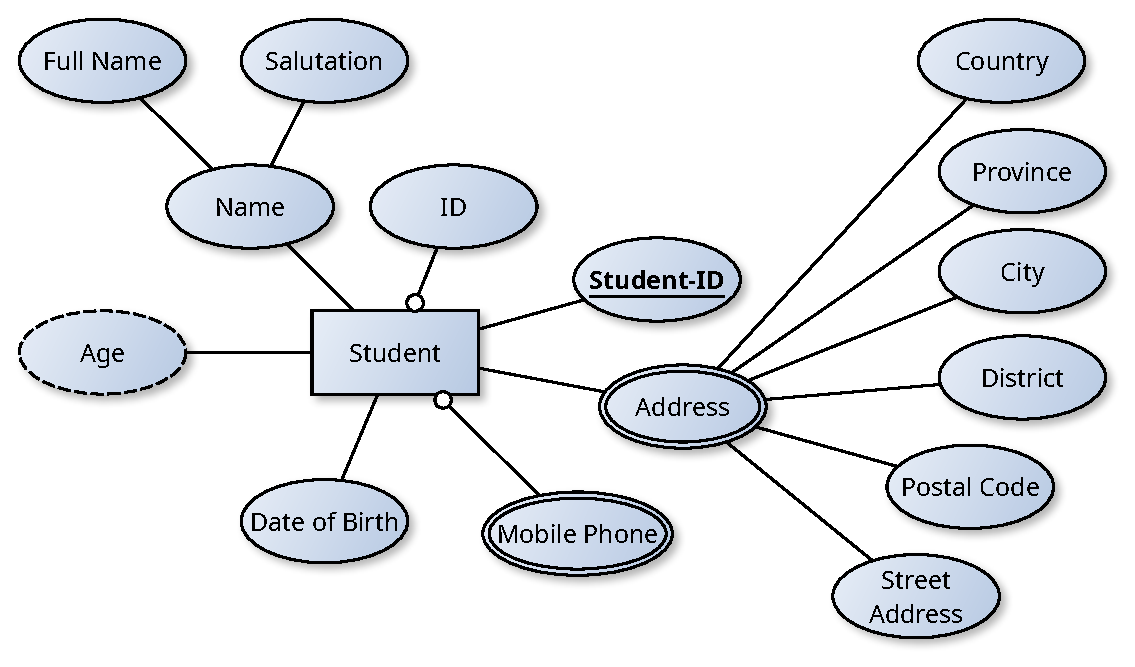
\includegraphics[scale=0.6]{\currentDir/erdStudent5}%
\caption{A new version of the \emph{Student} \pgls{ERD} from \cref{fig:erdStudent4}, this time with \emph{Student-ID} marked as primary key.}%
\label{fig:erdStudent5}%
\end{figure}%
%
While we feel very pessimistic about our idea about the concept of students, for now, we bravely march on and update our \pgls{ERD} from \cref{fig:erdStudent4}.
In the new \cref{fig:erdStudent5}, the attribute \emph{Student-ID} is marked as primary key.
This is done by underlining the attribute name~\cite{G2011EW2ITDS:CMUTERM}.%
%
\endhsection%
%
